\chapter{Emotions and physiological signals}
\label{ch:literature-physiological}

The empowerment of computers with the understanding of emotions is one of the focus of human-computer interaction research. The use of physiological signals of users in the process of detecting emotions involves the different input signals, such as electrocardiogram data, skin temperature and electro-dermal activity, among others. A significant number of works explore such inputs and the challenges associated with them on emotion recognition using physiological signals \parencite{jerritta2011physiological}.

% TODO: add Thesis - AIZoubi, page 62 (paper) or 79 (digital PDF indicator).
% TODO: add table info from Thesis - AIZoubi, page 45 (paper) or 62 (digital PDF indicator).

\begin{table}[h]
\caption{Most common psychophysiological measurements used in human interaction studies \parencite{jerritta2011physiological}}
\label{table:physiological-signals}
\begin{tabular}{L{.4\linewidth}L{.5\linewidth}}%
\toprule%
\textbf{Respiratiry system} & Breaths per minute\\
 & Respiration volume \\
\midrule
 \textbf{Electrodermal activity} & Skin conductance (SC) \\
 & Galvanic skin response (GSR) \\
\midrule
\textbf{Brain activity} & Electroencephalography (EEG) \\
& Brain imaging methods \\
\midrule
\textbf{Muscular system} & Electromyography \\
\midrule
\textbf{Cardiovascular system} & Heart rate variability (HRV) \\
& Respiratory Sinus Arrhythmia (RSA)  \\
& Cardiact output  \\
& Inter beat interval (IBI) \\
& Blood pressure (BP)  \\
\bottomrule%
\end{tabular}%
\end{table}

One of the reasons why physiological signals are interesting for emotion recognition is because suppressing emotions or social masking through physiological signals is impossible \parencite{kim2004emotion}. In the games research field, there have been studies aiming at using such theory and psychophysiological methods applied to game research \parencite{kivikangas2011review}. It has been demonstrated that it is possible to use physiological signals to automatically assess different emotional states in the context of games using a variety of signals \parencite{bousefsaf2013remote,yun2009game,rani2006empirical,tijs2008dynamic}.

Different approaches exists for emotion elicitation stimuli, feature extraction and classification methodologies regarding emotion recognition. Table \ref{table:physiological-signals} presents the most common psychophysiological measurements used in human interaction studies. The aim of this thesis is to remotely obtain physiological information from users to detect emotional states. As a consequence, the input signals presented in Table \ref{table:physiological-signals} were selected based on their potential to discriminate emotional states of users and the existence of techniques that are able to remotely and accurately measure them in a context involving games and natural behavior. HR was identified as a reliable physiological signal regarding emotion detection which can be remotely estimated via video of subjects. The use of HR has been confirmed by previous work, including its use for the measurement of emotional states \parencite{kivikangas2011review}, and detection of emotions as stress \parencite{choi2009using} and boredom \parencite{yamakoshi2007preliminary}. Additionally computer games were proven to provoke alteration in the mean HR of players at stressful periods of gameplay \parencite{sharma2006assessment,rodriguez2015vr}, which makes HR an ideal signal for the method presented in this thesis.

The following sections present more details regarding the physiology of HR and its use in emotion detection.

%Multimodal sensing consists of reading different signal channels from a subject. A person presents a wide set of those channels, such as blood pressure, pulse oximetry, facial expressions, pupillary variation, among others. The analysis of such data can be used to infer the subject's emotional/stress state, for instance. Usually biometric sensors attached to the subject are used to read the channels, however remote approaches are proving to be feasible. The following subsections present some of those channels and the sensing techniques used to extract them. All of them are non-intrusive, working by analyzing a video of the subject with no physical contact.

%In games research, quantitative approaches already used HR to measure engagement \parencite{ravaja20051}, for instance.
%there are initiatives to measure such states and other elements, such as engagement/immersion \parencite{boyle2012engagement} and presence \parencite{weibel2011immersion}.

%%%%%%%%%%%%%%%%%%%%%%%%%%%%%%%%%%%%%%%%%%%%%%%%%%%%%%%%%%%%%%%%%%%%%%%%%%%%%%%%%%%%%%%%%%%%%%%%%%%%%%%
\section{Physiology of heart rate}
%%%%%%%%%%%%%%%%%%%%%%%%%%%%%%%%%%%%%%%%%%%%%%%%%%%%%%%%%%%%%%%%%%%%%%%%%%%%%%%%%%%%%%%%%%%%%%%%%%%%%%%

The cardiac cycle is periodic and it contains a set of waves that reflect depolarization and repolatization events, which are all connected to the functioning mechanism of the heart \parencite{yanowitz2012introduction}. Figure \ref{fig:rr-interval} illustrates two cardiac cycles with highlights on each of such waves. The x-axis represents time in milliseconds and the y-axis represent the wave amplitude. A heartbeat is a contraction and relaxation of the heart, which is connected to the Q, R and S waves, known as the QRS complex.

\begin{figure}[h!]
    \centering
    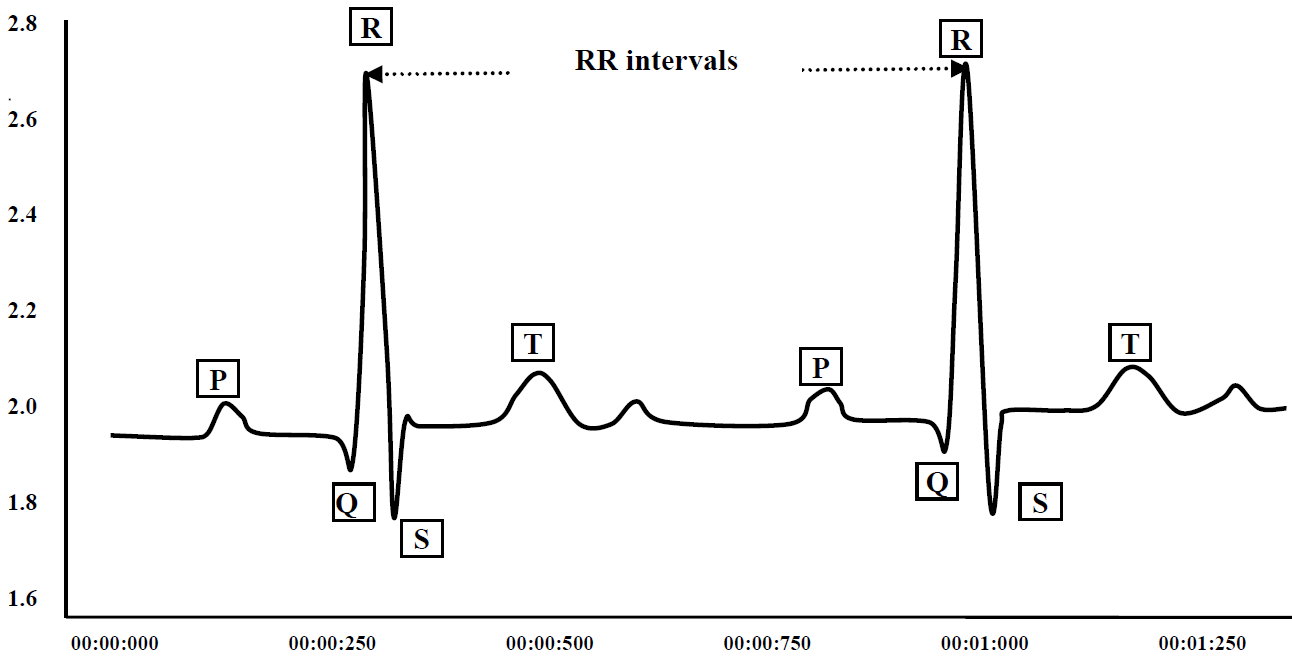
\includegraphics[width=1.0\linewidth]{Content/figures/rr-interval.png}
    \caption{Two cardiac cycles with highlights on each its electrical waves. The X axis represents time in milliseconds and the Y axis represent the wave amplitude. A heartbeat is connected to the Q, R and S waves, known as the QRS complex. Reproduced from \textcite{ahmed2010heart}.}
    \label{fig:rr-interval}
\end{figure}

The tracing of the QRS complex allows the monitoring of the heart rate. The peak of the R wave, referred to as R peak, marks an specific time in the cardiac cycle. The difference between two R wave peaks is the RR interval, also known as inter-beat interval (IBI). The RR interval reflects the entire duration of each heart beat. As a consequence, the amount of R waves within one minute is used to calculate the HR. The variations in time between R peaks, which is the beat-to-beat variability of HR, is referred to as heart rate variability (HRV).

The HR is connected to the central nervous system and it can be influenced by a series of different elements, including modifiable and non-modifiable ones \parencite{valentini2009variables}. Modifiable elements are those related to external influence, such as mental stress or physical activity. Non-modifiable elements are related to physiology, such as age, gender and race. A healthy human adult has a HR within the interval of [45 bpm, 240 bpm], the equivalent of [0.75 Hz, 4 Hz] \parencite{li2014remote}.

% A healthy human adult has a HR between 45 - 240 bpm (0.75 - 4 Hz) [1]. There are many factors influencing the HR of a person, both modifiable (e.g. physical activity, mental stress, smoking) and non-modifiable (e.g. age, gender) [12]. The HR can change rapidly from activities such as postural changes [13] and also from uncontrolled events such as cardiac arrhythmia and sudden cardiac arrest [14, 15].

% [1] X. Li et al. “Remote Heart Rate Measurement from Face Videos under Realistic Situations”. In: Computer Vision and Pattern Recognition (CVPR), 2014 IEEE Conference on. June 2014, pp. 4264–4271. doi: 10.1109/CVPR.2014.543
%
% [12] M. Valentini and G. Parati. “Variables Influencing Heart Rate”. In: Progress in Cardiovascular Diseases 52 (2009), pp. 11–19
%
% [13] C. Borst et al. “Mechanisms of initial heart rate response to postural change”. In: American Journal of Physiology - Heart and Circulatory Physiology 243.5 (1982), H676–H681
%
% [14] National Heart, Lung and Blood Institute. How Is Sudden Cardiac Arrest Diagnosed? http://www.nhlbi.nih.gov/health/health-topics/topics/ scda/diagnosis. Accessed: 2016-06-02

%%%%%%%%%%%%%%%%%%%%%%%%%%%%%%%%%%%%%%%%%%%%%%%%%%%%%%%%%%%%%%%%%%%%%%%%%%%%%%%%%%%%%%%%%%%%%%%%%%%%%%%
\section{Heart rate, stress and frustration}
%%%%%%%%%%%%%%%%%%%%%%%%%%%%%%%%%%%%%%%%%%%%%%%%%%%%%%%%%%%%%%%%%%%%%%%%%%%%%%%%%%%%%%%%%%%%%%%%%%%%%%%

The foundation of HR-based approaches for emotional estimation draws on the theory that physiological signals are linked to emotion regulation \parencite{appelhans2006heart,fenton2012emotion,schubert2009effects}. The automatic nervous system (ANS), a key system in the generation of physiological arousal \parencite{appelhans2006heart}, is subdivided into the sympathetic nervous system (SNS) and the parasympathetic nervous system (PNS). Those systems interact (often antagonistically) to produce variations in the physiological signals to prepare a person to react to a situation. The SNS is dominant during physical and psychological stress, triggering the body to alertness, increasing HR, for instance. This is commonly referred to as ``fight or flight'' response. The PNS, on the other hand, is dominant in periods of stability and relative safety, maintaining physiological signals at a lower degree of arousal, e.g. decreasing HR. The continuous changes between SNS and PNS impulses cause variations of HR and HRV \parencite{schubert2009effects}, which refers to beat-to-beat alternations in HR intervals.

Physiological signals, such as HR, are hard to fake because of their link with the ANS, differently from facial expressions \parencite{Landowska}, for instance. As a consequence, HR and its derivatives, such as HRV, have been used as reliable sources of information in different emotion estimation methods \parencite{kukolja2014comparative}. Additionally it has been used as an indication of perceived interest and confusion in mobile applications \parencite{xiao2015towards}, as player input for games \parencite{stockhausen2013beats}, and as triangulation of phychophysiological emotional reactions to digital media stimuli \parencite{nogueira2015annotation}. The significant variation of physiological signals, however, is an obstacle to its use in emotional estimation. Signals increase during emotional arousal, but decrease in response to attention engagement, which makes the measurement of engagement, for instance, a non-trivial process \parencite{ravaja20051}. Despite such challenges, the use of HR and HRV has been demonstrated in a continuous arousal monitor \parencite{grundlehner2009design} as well as a detection mechanism for mental and physical stress based on physical and mental tasks \parencite{vandeput2009heart,garde2002effects}. Results indicate higher HR during the mentally demanding task when compared to the rest period. The HR mean alone also has been shown to be a measurement of frustration in a game \parencite{rodriguez2015vr}.

%As previously mentioned, however, the use of sensors that require physical contact might disturb the user experience or be sensitive to noise. Even when users state they forgot about the use of physical sensors during a gaming session, researchers still face noisy data due to subject motion affecting the sensors \parencite{brogni2006variations}.

\textcite{vandeput2009heart} demonstrate the use of HR and HRV to detect mental and physical stress. Three demanding activities (a postural task, a mental task and a task that is a combination of both) are used and for almost all HR measures obtained, the demanding activities can be distinguished from the rest period. The authors also point out that mental stress decreased high frequency components of the HRV interval (i.e. $HRV_{HF}$), while increasing low frequency ones (i.e. $HRV_{LF}$). A similar experiment was conducted by \textcite{garde2002effects} involving two tasks: one being mental and physically demanding (digital version of the Stroop color word test \parencite{golden1978stroop}) and other being only physically demanding. The authors confirm the findings of \textcite{vandeput2009heart} by showing higher HR, increased $HRV_{LF}$ and decreased $HRV_{HF}$ during the mentally demanding task when compared to the rest period.

\textcite{bousefsaf2013remote} also use a digital version of the Stroop test in a similar experiment. A combination of HR, HRV and HRV\textsubscript{HF} is used to estimate the stress state of subjects. The resulting stress state curve tends to decrease during the rest period and increase during stress sessions (as did the HR), in accordance with the previously mentioned works; additionally the self-reported answers to questionnaires present significant differences of stress level in the rest and in the stress sessions as well. \textcite{mcduff2014remote,mcduffcogcam} also use HR and its variants in order to measure cognitive stress during computer tasks. According to the authors, the average heart rate and breathing rate are not significantly different in any case, which differs from the findings of previously mentioned work. The variations of HRV\textsubscript{LF} and HRV\textsubscript{HF}, however, are significantly different during the cognitive tasks compared to the rest period; higher HRV\textsubscript{LF} and lower HRV\textsubscript{HF} power are found in both cognitive tasks compared to the rest period, which aligns with findings of previous work. Stress predictions made by the model are consistent with the self-reported answers provided by subjects.

\textcite{grundlehner2009design} present a real-time, continuous arousal monitor. Using a wireless sensor network for signal acquisition, the authors record and use four signals from subjects to estimate arousal: electrocardiogram (ECG), respiration, skin conductance and skin temperature. The ECG is used to calculate HRV, which is then used in the estimation. A regression analysis is performed to identify the importance of the features in the estimation of arousal. HRV\textsubscript{LF} and HRV\textsubscript{HF} are not significant when compared to the other signals (e.g. skin conductance), while the standard deviation of HRV presents a significant weight. The arousal prediction matches the hypothesized arousal events marked by the authors in each of the experiment parts (e.g. start of noise in the audio part).

% TODO: add \cite{anttonen2005emotions,witvliet2007play}
